\documentclass[
  11pt,
  letterpaper,
   addpoints,
   answers
  ]{exam}

\usepackage{../exercise-preamble}

\begin{document}

\noindent
\begin{minipage}{0.47\textwidth}

\includegraphics[width=\textwidth]{../fcfm_die}
\end{minipage}
\begin{minipage}{0.53\textwidth}
\begin{center} 
\large\textbf{Fundamentos de control de sistemas} (EL4111-1) \\
\large\textbf{Clase auxiliar 6s} \\
\small Prof.~Roberto Cardenas Dobson\\
\small Prof.~Aux.~Osvaldo Jimenez - Erik Sáez\\
\small Ayudantes.~Simon Arenas- Juan Pablo Baez - Francisco Garces - Sofia Ibarra\\
\end{center}
\end{minipage}

\vspace{0.5cm}
\noindent
\vspace{.85cm}

\begin{questions}
%----------------------------------------------
    \question Para la planta de segundo orden:
    \begin{align}
        G(s) = \frac{3}{s^2 + 1}
    \end{align}
   Se desea llevar los polos de lazo cerrado al punto de operación \( -1 \pm j \sqrt{3} \). Sabiendo esto:
    \begin{enumerate}
        \item Diseñe un controlador que elimine la sobresoscilación en la planta y entregue cero error en estado estacionario para una entrada escalón. Considere el uso de cancelación.
        \item Rediseñe el sistema considerando ahora un anti-windup en su diseño. ¿Para qué sirve esto?
    \end{enumerate}
%----------------------------------------------
\begin{solution}
    \subsection*{Resolucion 1.1}
    Se buesca realizar un controlador tal que elimine la sobresoscilacion y entregue cero error en estado estacionario para entrada escalon. Debido a que se nos pide el eliminar la sobre-oscilacion, pero se nos entrega el punto de diseño se priorizara este ultimo, ademas el controlador tiene que hacer uso de cancelacion, por tanto se propone lo siguiente:
    \begin{align}
        G_{c}(s)= K_{c}\frac{(s^{2}+1)}{s(s+a)}
    \end{align}
    Esto con el fin de que se cumpla la condicion de cancelacion,esto permite que se obtenga como variable libre el parametro a, el cual debe ser sintonizado en base a la condicion de angulo,por lo tanto se realiza un esquema de LGR tal que:
    \begin{center}
        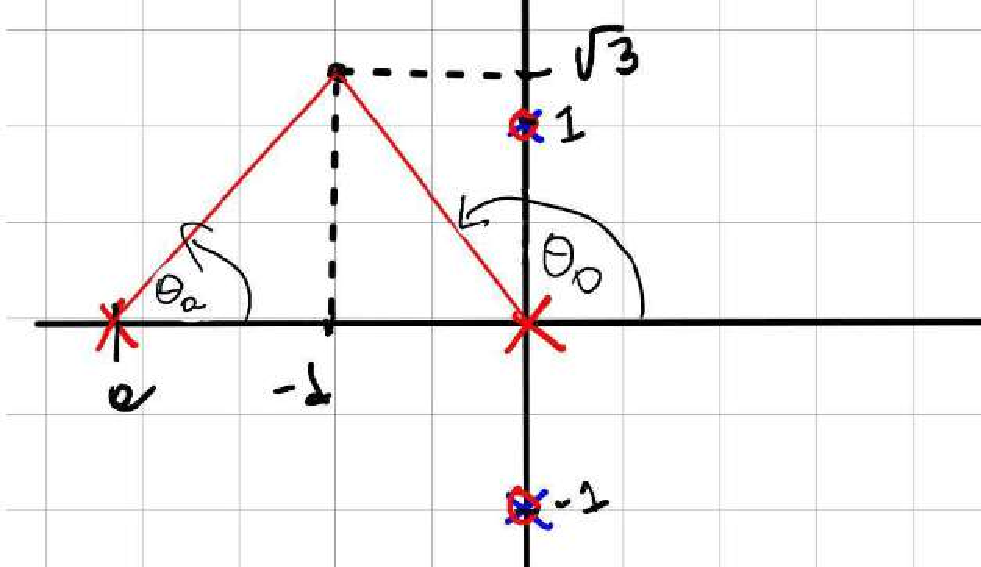
\includegraphics[width=0.5\textwidth]{Auxiliar_6_13}
        \captionof{figure}{LGR del esquema.}
    \end{center}
    Por lo que se tiene de manera directa que se debera cumplir que:
    \begin{align}
        \theta_{a} + \theta_{0} = 180^{\circ} 
    \end{align}
    Se obtiene que $\theta_{0}$
    \begin{align}
        \theta_{0} = 180^{\circ}- atan\left(\frac{\sqrt{3}}{1}\right) = 120^{\circ}
    \end{align}
    Con lo que se obtiene que para $\theta_{a}=60^{\circ}$, lo que implica que $a$ se encuentra a la izquierda del punto de diseño y este tiene un valor:
    \begin{align}
        \frac{\sqrt{3}}{a-1}&= tan(60^{\circ})\\
        a&= 2
    \end{align}
    Luego se debe determinar el valor de la ganancia $K_{c}$,para esto se debe cumplir la condicion de modulo que vendra caracterizada por:
    \begin{align}
        K_{c} &= \abs{\frac{1}{G_{p}(s)G_{c}(s)H(s)}}_{s=s^{*}}\\
              &= \abs{\frac{1}{\frac{3}{s^{2}+1}\frac{s^{2}+1}{s(s+2)}}}_{s=-1+j\sqrt{3}}\\
              &= \abs{\frac{1}{\frac{3}{s(s+2)}}}_{s=s^{*}}\\\
              &= \frac{4}{3}
    \end{align}
    Con lo que finalmente se tendra que el controlador sera de la forma:
    \begin{align}
        G_{c}(s) = \frac{4}{3}\frac{s^{2}+1}{s(s+2)}
    \end{align}
    \subsection*{Resolucion 1.2}
    Ahora nuestro sistema debera considerar el efecto del Anti-Windup,la funcion de este es limitar la accion integral del controlador cuando este se encuentra en saturacion, es decir que el controlador entrege una señal que no puede ser aplicada al sistema (\textit{Puedes pensar en que una valvula abra mas alla de un 100\%}), esto se logra entender de mejor manera en los siguientes graficos:
    \begin{center}
        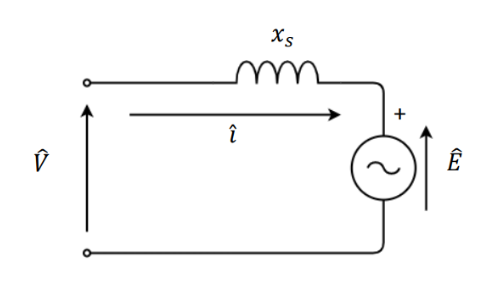
\includegraphics[width=0.7\textwidth]{Auxiliar_6_2}
        \captionof{figure}{Podemos ver a la izquierda la salida del sistema y del controlador sin Anti-Windup y a la derecha con Anti-Windup, para el primer caso por ejemplo si fuera un voltaje o corriente podria producir un daño en el sistema, por lo que el Anti-Windup limita la señal de control para que no se sature el sistema.}
    \end{center}
    Si bien se soluciona el problema de la saturacion, debemos tener en cuenta que la salida del sistema tambien se vera afectada, esto se visualiza en lo siguiente:
    \begin{center}
        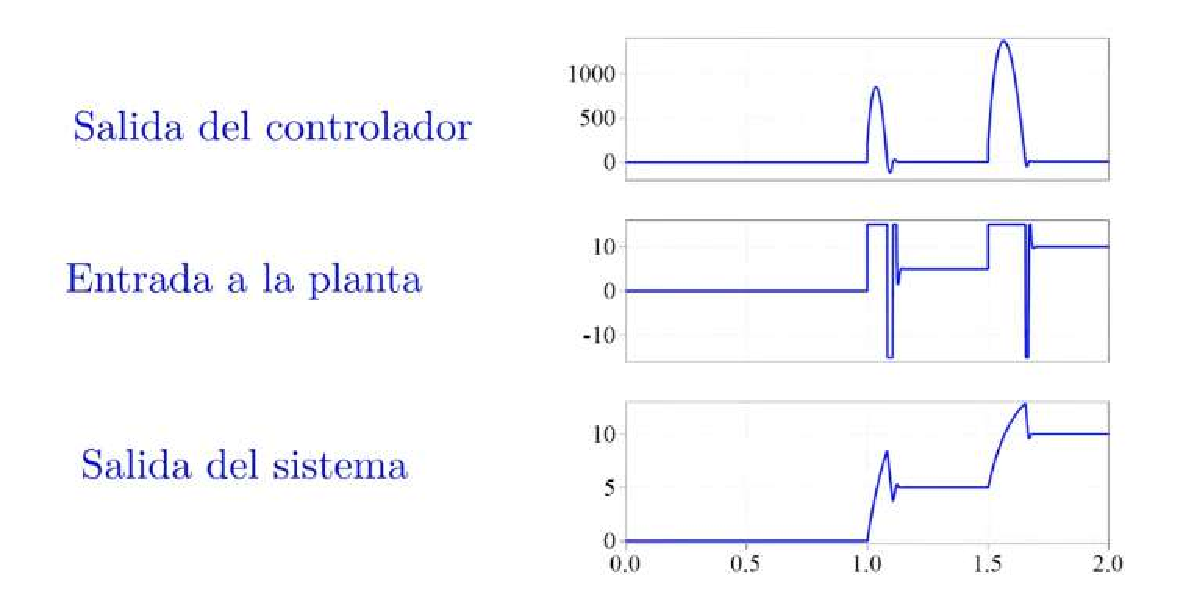
\includegraphics[width=0.7\textwidth]{Auxiliar_6_3}
        \captionof{figure}{Se ve que la salida del sistema se ve afectada debido al efecto del saturador.}
    \end{center}
    \begin{center}
        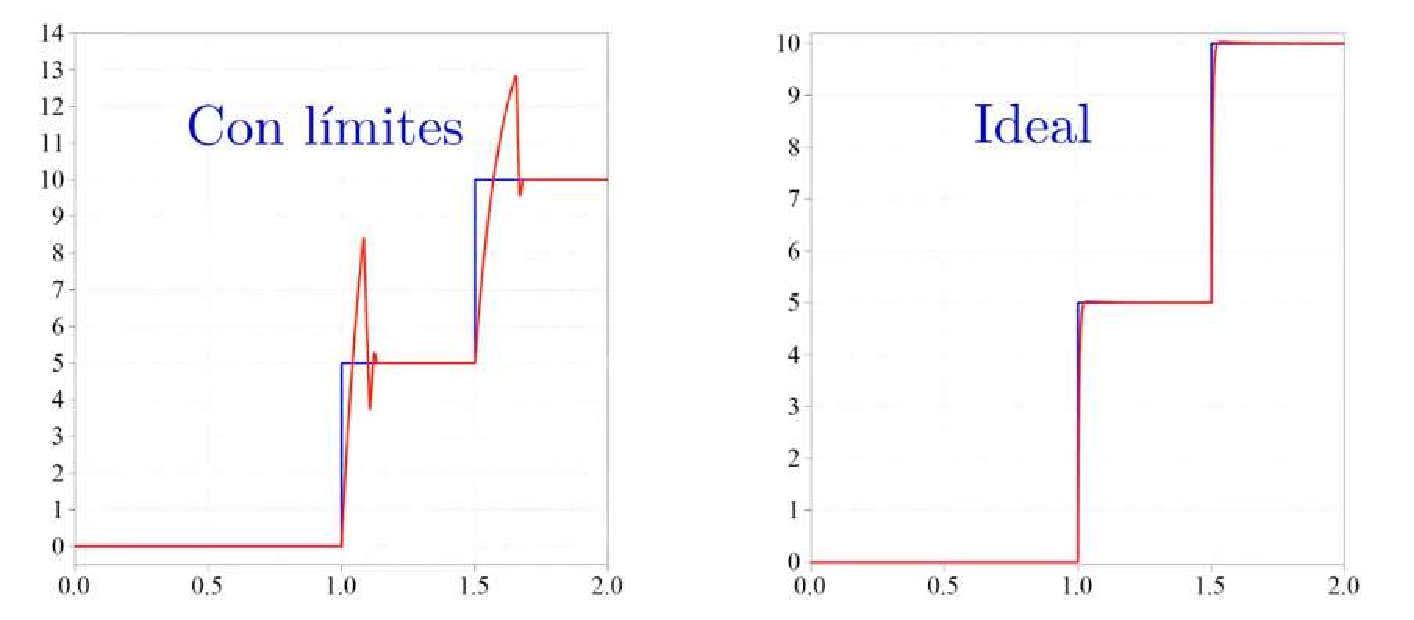
\includegraphics[width=0.7\textwidth]{Auxiliar_6_4}
        \captionof{figure}{Se observa la comparacion entre un sistema con saturacion y un sistema sin saturador ideal.}
    \end{center}
    Por lo que se busca eliminar el efecto integrador,esto se visualiza en la siguiente figura:
    \begin{center}
        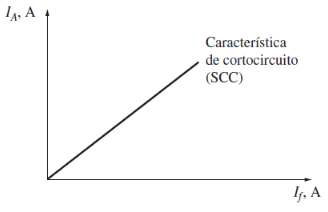
\includegraphics[width=0.7\textwidth]{Auxiliar_6_5}
        \captionof{figure}{Implementación del esquema de anti-windup propuesto para
        controladores con funciones de transferencias que son bipropias.}
    \end{center}
    Luego deberemos obtener $K^{\infty}$ el cual se define como:
    \begin{align}
        K^{\infty} &= \lim_{s\to \infty}G_{c}(s)\\
                   &= \lim_{s\to \infty} \frac{4}{3}\frac{s^{2}+1}{s(s+2)}\\
                   &= \frac{4}{3}
    \end{align}
    Sabiendo que $K(s)^{-1} = G_{c}(s)^{-1}$ se obtiene que:
    \begin{align}
        G_{c}(s)^{-1} &= \frac{3}{4}\frac{s(s+2)}{s^{2}+1} 
    \end{align}
    De esta manera se obtiene que:
    \begin{align}
        K(s)^{-1} - (K^{\infty})^{-1} &= \frac{3}{4}\frac{s(s+2)}{s^{2}+1} - \frac{4}{3}\\
        &=\frac{3}{4}\cdot \frac{2s-1}{s^{2}+1}
    \end{align}
    De esta manera se obtiene que el esquema vendra dado por: 
    \begin{center}
        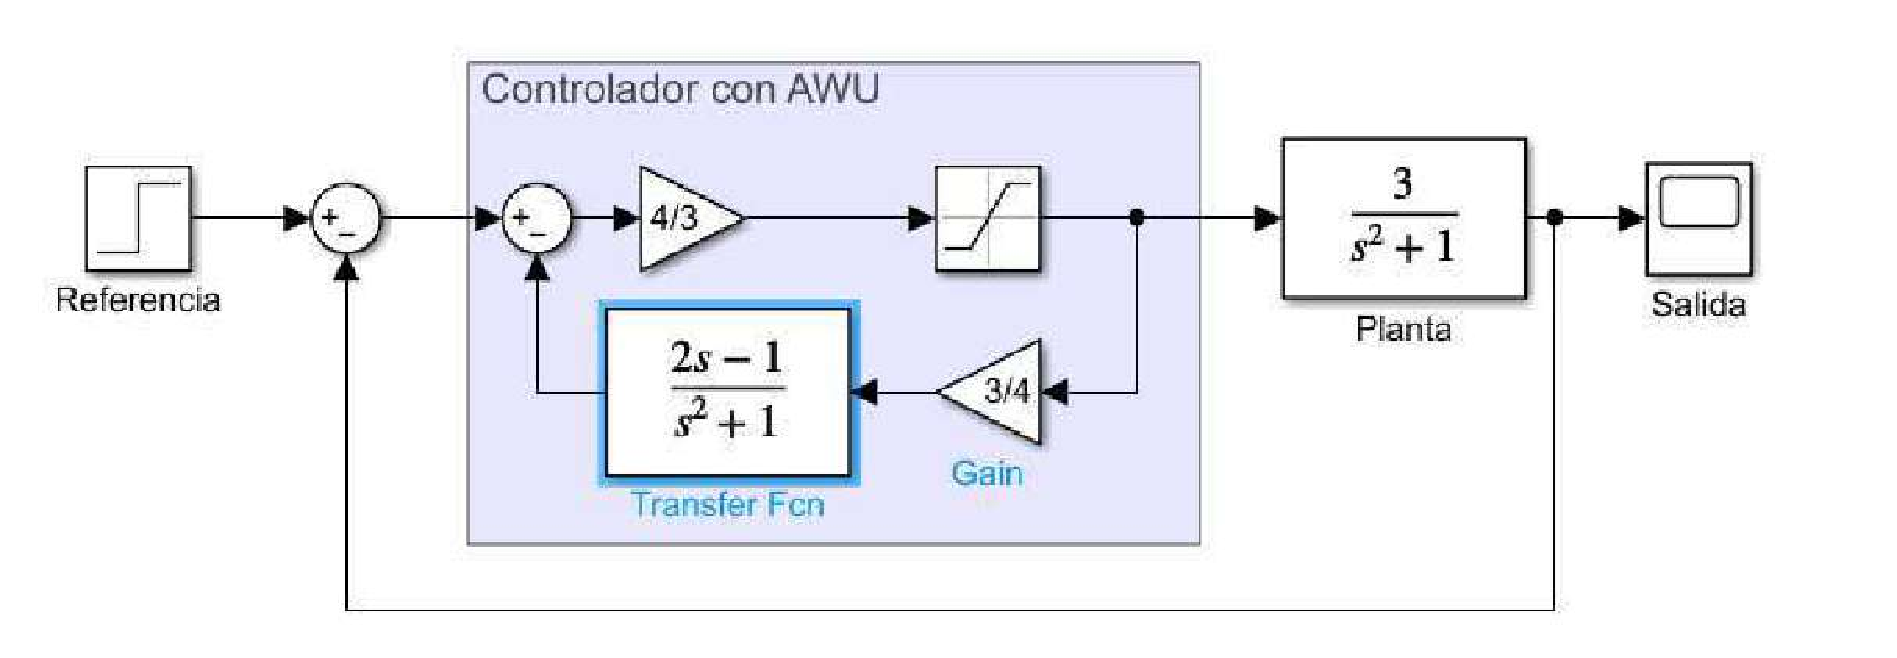
\includegraphics[width=0.7\textwidth]{Auxiliar_6_14}
        \captionof{figure}{Implementación del esquema de anti-windup propuesto para
        controladores con funciones de transferencias que son bipropias.}
    \end{center}
    \end{solution}
%----------------------------------------------
    \question Suponga que tiene el estanque de la Figura 1, en donde la altura del agua es controlada por medio de una válvula que deja pasar una mayor o menor cantidad de agua proveniente de la bomba. Asuma que este sistema puede ser descrito por la siguiente ecuación:
    \begin{align}
        G(s) = \frac{16(s + 3)}{(s + 5)(s^2 + 6s + 10)}
    \end{align}
    \begin{center}
        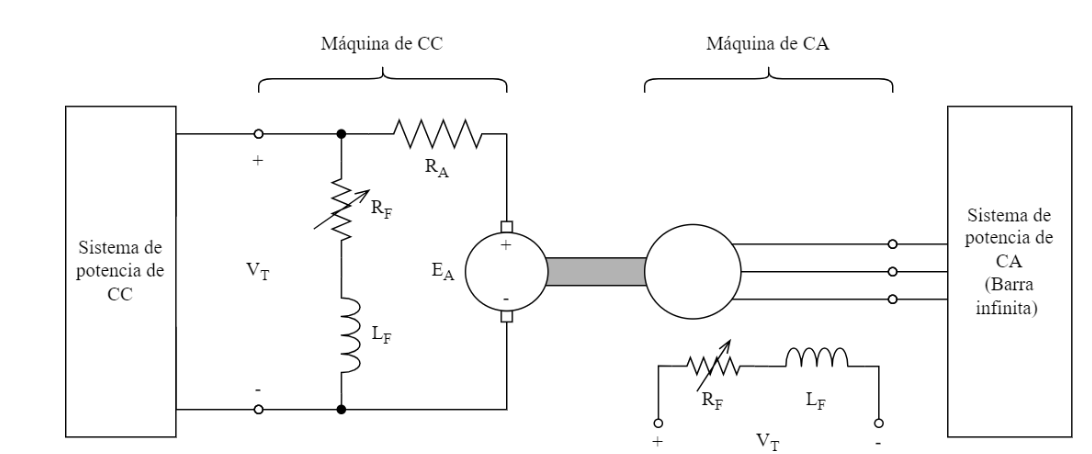
\includegraphics[width=0.5\textwidth]{Auxiliar_6_1}
        \captionof{figure}{Esquema }
    \end{center}
    \begin{enumerate}
        \item Cree un controlador que estime convenientemente para una frecuencia \(\omega_n = 2 \, \text{rad/s}\) y un coeficiente de amortiguamiento de 0.7. Justifique por qué va a utilizar el controlador que eligió.
        \item  Dado el constante uso del estanque, la válvula se ha desgastado, lo que provoca un retardo de transporte de 0.02 [s]. Utilizando la aproximación de Padé, modifique el controlador creado en (a) para suplir este cambio en la planta.
        \item ¿Es posible rediseñar el sistema considerando ahora un anti-windup? ¿Para qué sirve esto? Dibuje el esquema de control al utilizar esta técnica.
    \end{enumerate}
%----------------------------------------------
\begin{solution}
\subsection*{Resolucion 2.1}
Se busca obtener un controlador tal que su frecuencia natural sea de 20 rad/s y su coeficiente de amortiguamiento sea de 0.7, por lo que se debe obtener su punto de diseño, en esta ocacion se hara uso de la formula:
\begin{align}
    s_{1,2}^{*} &= -\zeta \omega_{n} \pm j\omega_{n}\sqrt{1-\zeta^{2}}\\
    &= -0.7\cdot 2 \pm j2\sqrt{1-0.7^{2}}\\
    &= -1.4 \pm j1.43
\end{align}
Notamos que existe una libre eleccion en cuanto a que controlador tomar, es decir que podemos usar por ejemplo un PI o un PID,se optara por el primero por ser mas simple al implementar, pero por ejemplo con un PID se podria cancelar el termino cuadratico del denominador.Por lo tanto se tiene que:
\begin{align}
    G_{c}(s) = K_{c}\cdot \frac{(s+a)}{s}
\end{align}
Luego se debera cumplir la condicion de angulo por lo que realizando un LGR se obtiene lo siguiente:
\begin{center}
    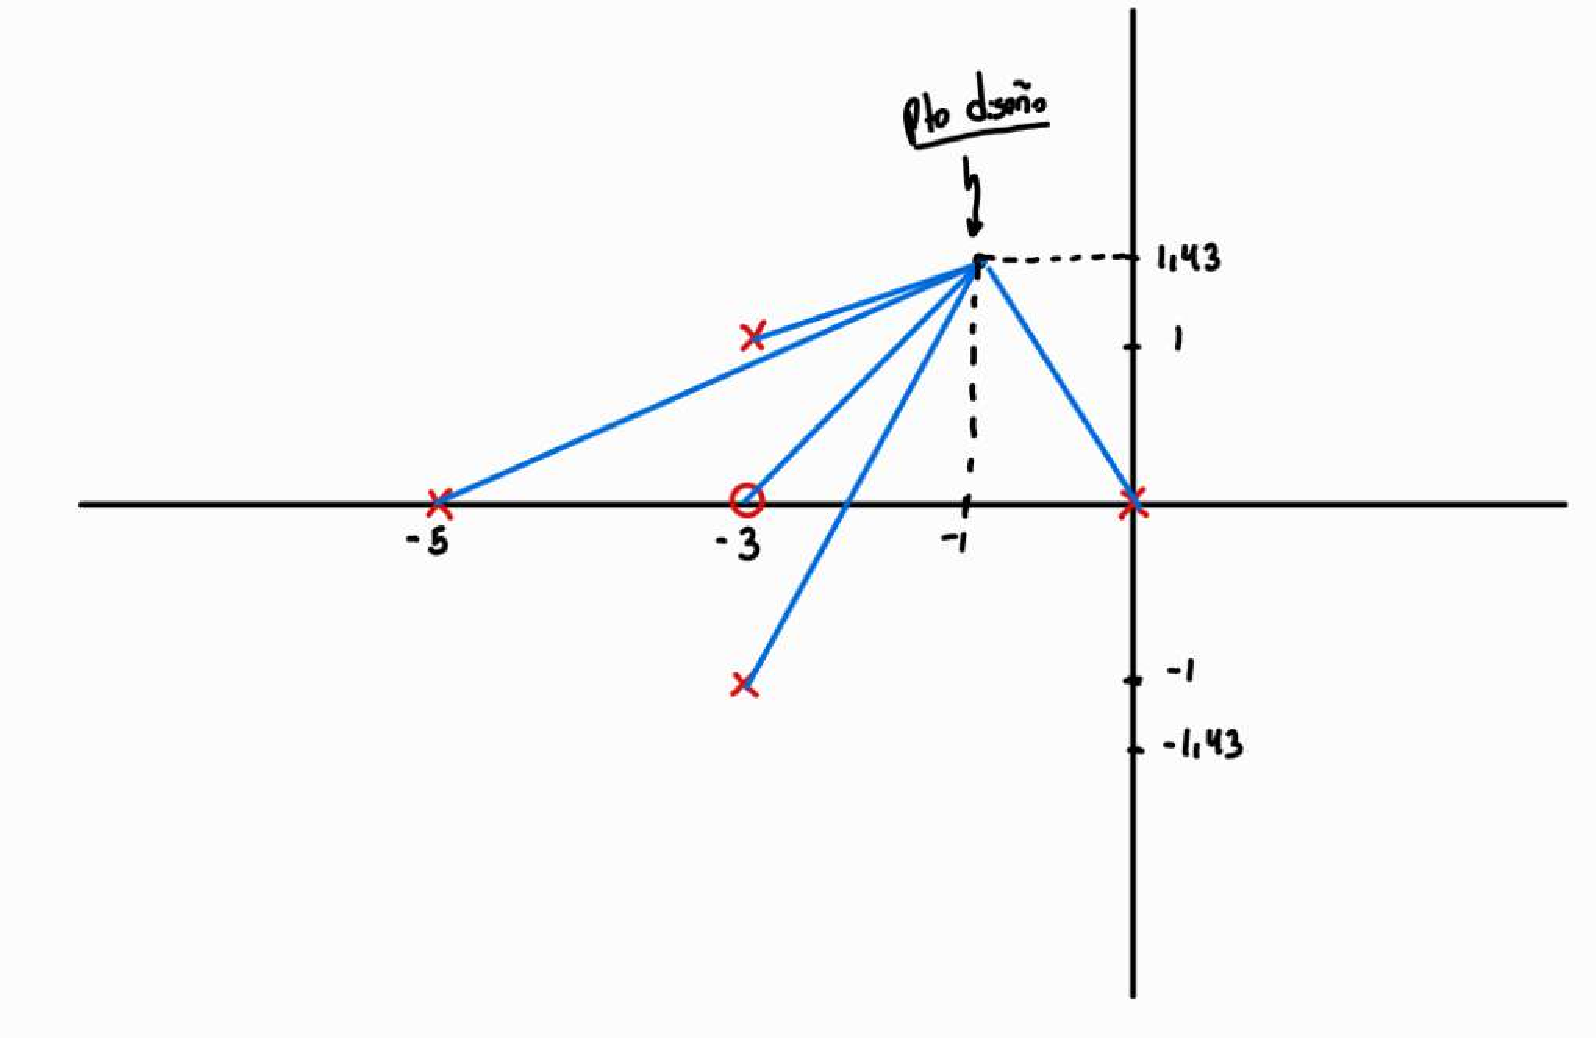
\includegraphics[width=0.6\textwidth]{Auxiliar_6_15}
    \captionof{figure}{LGR del lazo anterior.}
\end{center}
De esta manera identificamos que se debe cumplir:
\begin{align}
    \sum \theta_{0} - \sum \theta_{z} = 180^{\circ}
\end{align}
Por lo que analizando cada uno de estos, tenemos que:
\begin{align}
    \theta_{0} &= 180^{\circ} - atan\left(\frac{1.43}{1.4}\right) = 134.39^{\circ}\\
    \theta_{5} &= atan\left(\frac{1.43}{5-1.14}\right) = 21.66^{\circ}\\
    \theta_{3} &= atan\left(\frac{1.43}{3-1.14}\right) = 41.78^{\circ}\\
    \theta_{-3+j} &= atan\left(\frac{1.43-1}{3-1.4}\right) = 15.04^{\circ}\\
    \theta_{-3-j} &= atan \left(\frac{1.43+1}{3-1.4}\right)= 56.64^{\circ}
\end{align}
Por lo que de esta manera se obtiene que:
\begin{align}
    \sum \theta_{0} - \sum \theta_{z} = 180^{\circ}\\
    \theta_{0} + \theta_{5} + \theta_{-3+j} + \theta_{-3-j} - \theta_{3} - \theta_{a} = 180^{\circ}\\
    134.39 + 21.66 + 15.04 + 56.64 - 41.78 - \theta_{a} = 180^{\circ}\\
    \theta_{a}  = 5.95^{\circ} 
\end{align}
Con lo que ya es posible el determinar el valor de a, ademas notamos que este valor no indica que se debera ubicar a la izquierda del punto de diseño y ademas encontrarse alejado de este.
\begin{align}
    tan(5.95^{\circ}) = \frac{1.43}{a-1.4}\\
\end{align}
Con lo que se tiene que $a = 15.121$, se debe obtener unicamente el valor de la ganancia $K_{c}$, para esto se debe cumplir la condicion de modulo, por lo que se tiene que:
\begin{align}
    K_{c} &= \abs{\frac{1}{G_{p}(s)G_{c}(s)H(s)}}_{s=s^{*}}\\
          &= \abs{\frac{1}{\frac{16(s+3)}{(s+5)(s^{2}+6s+10)}\frac{s+15.121}{s}}}_{s=-1.4+j1.43}\\
          &= \abs{\frac{1}{\frac{16(s+3)}{(s+5)(s^{2}+6s+10)}\frac{s+15.121}{s}}}_{s=s^{*}}\\
          &= 0.0789
\end{align}
Finalmente se tendra que el controlador sera de la forma:
\begin{align}
    G_{c}(s) = 0.0789\frac{s+15.121}{s}
\end{align}
%----------------------------------------------
\subsection*{Resolucion 2.2}
Se busca obtener un controlador que permita suplir el retardo de transporte de 0.02s, por lo que se debe obtener el controlador que permita suplir este retardo,este retardo se puede interpretar matematicamente como:
\begin{align}
    G(s) = e^{-Ts}
\end{align}
Donde T es el retardo en segundo, sabemos que la senal no cambiara su forma pero si se retardara los T segundos.
\begin{center}
    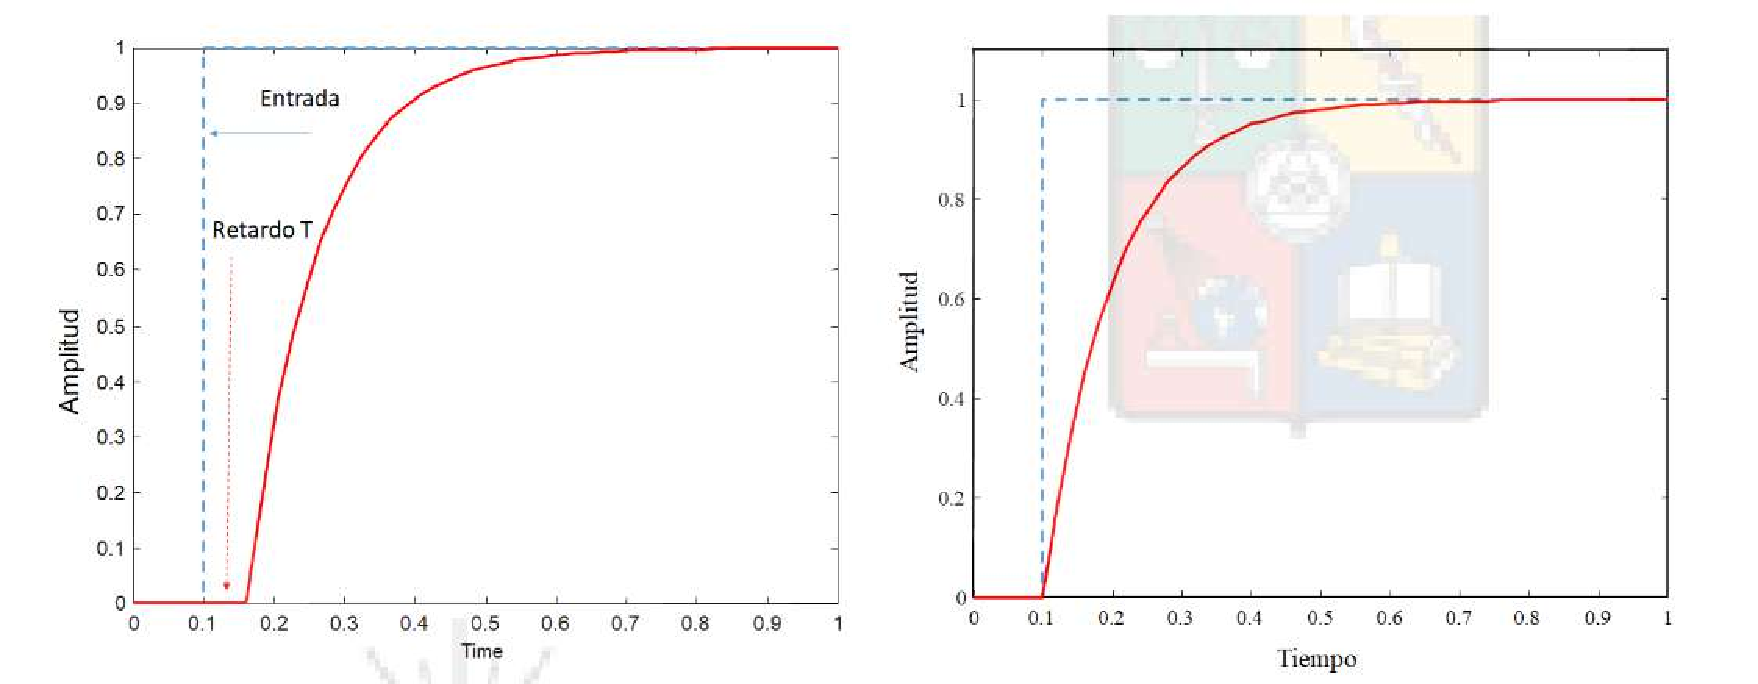
\includegraphics[width=0.8\textwidth]{Auxiliar_6_6}
    \captionof{figure}{A la izquierda se observa la salida del sistema considerando un retardo de T segundos mientras que a la derecha se tiene la salida sin retardo.}
\end{center}
Por lo que una planta la cual considera el retardo se tendra que:
\begin{align}
    G_{p}(s)= \frac{a}{s+a} e^{-Ts}
\end{align}
Observamos que el implementar un controlador de la forma anterior resulta bastante complejo, es por esto que se da uso a la aproximacion de Pade, en particular utilizaremos la de primer orden la cual se define como:
\begin{align}
    e^{-Ts} \approx \frac{1-Ts/2}{1+Ts/2}
\end{align}
y de esta maenra ya es implementable.Para el caso particular del problema tenemos que:
\begin{align}
    e^{-0.02s} \approx \frac{1 - \frac{s \cdot 0.02}{2}}{1 + \frac{s \cdot 0.02}{2}} = \frac{100 - s}{100 + s}
\end{align}
Con lo que la planta con retardo vendra dada por
\begin{align}
    G_{p}(s) \approx \frac{16(s+3)}{(s+5)(s^{2}+6s+10)}\cdot \frac{100-s}{100+s}
\end{align}
Luego re-escribe la aproximacion tal como:
\begin{align}
    G_{p}(s) \approx \frac{16(s+3)}{(s+5)(s^{2}+6s+10)}\cdot -\frac{s-100}{s+100}
\end{align}
Donde notamos dos aspectos importantes a considerar:
\begin{enumerate}
    \item Se tiene que el cero y el polo producido por el retardo se encuentran bastante lejanos, por lo que a pesar de que debemos considerar su aporte, este sera practicamente despreciable.
    \item Se debe tener muy en cuenta que el retardo nos introduce un signo negativo en el sistema, por lo que se debe tener en cuenta al momento de realizar el diseño del controlador,dado que cambiara las condiciones de angulo y modulo.
\end{enumerate}
Dado que ahora tenemos un signo negativo, la condicion de angulo vendra dada por:
\begin{align}
    \sum \theta_{0} - \sum \theta_{z} = 0^{\circ}
\end{align}
Tenemos por tanto que el nuevo LGR vendra dado por:
\begin{center}
    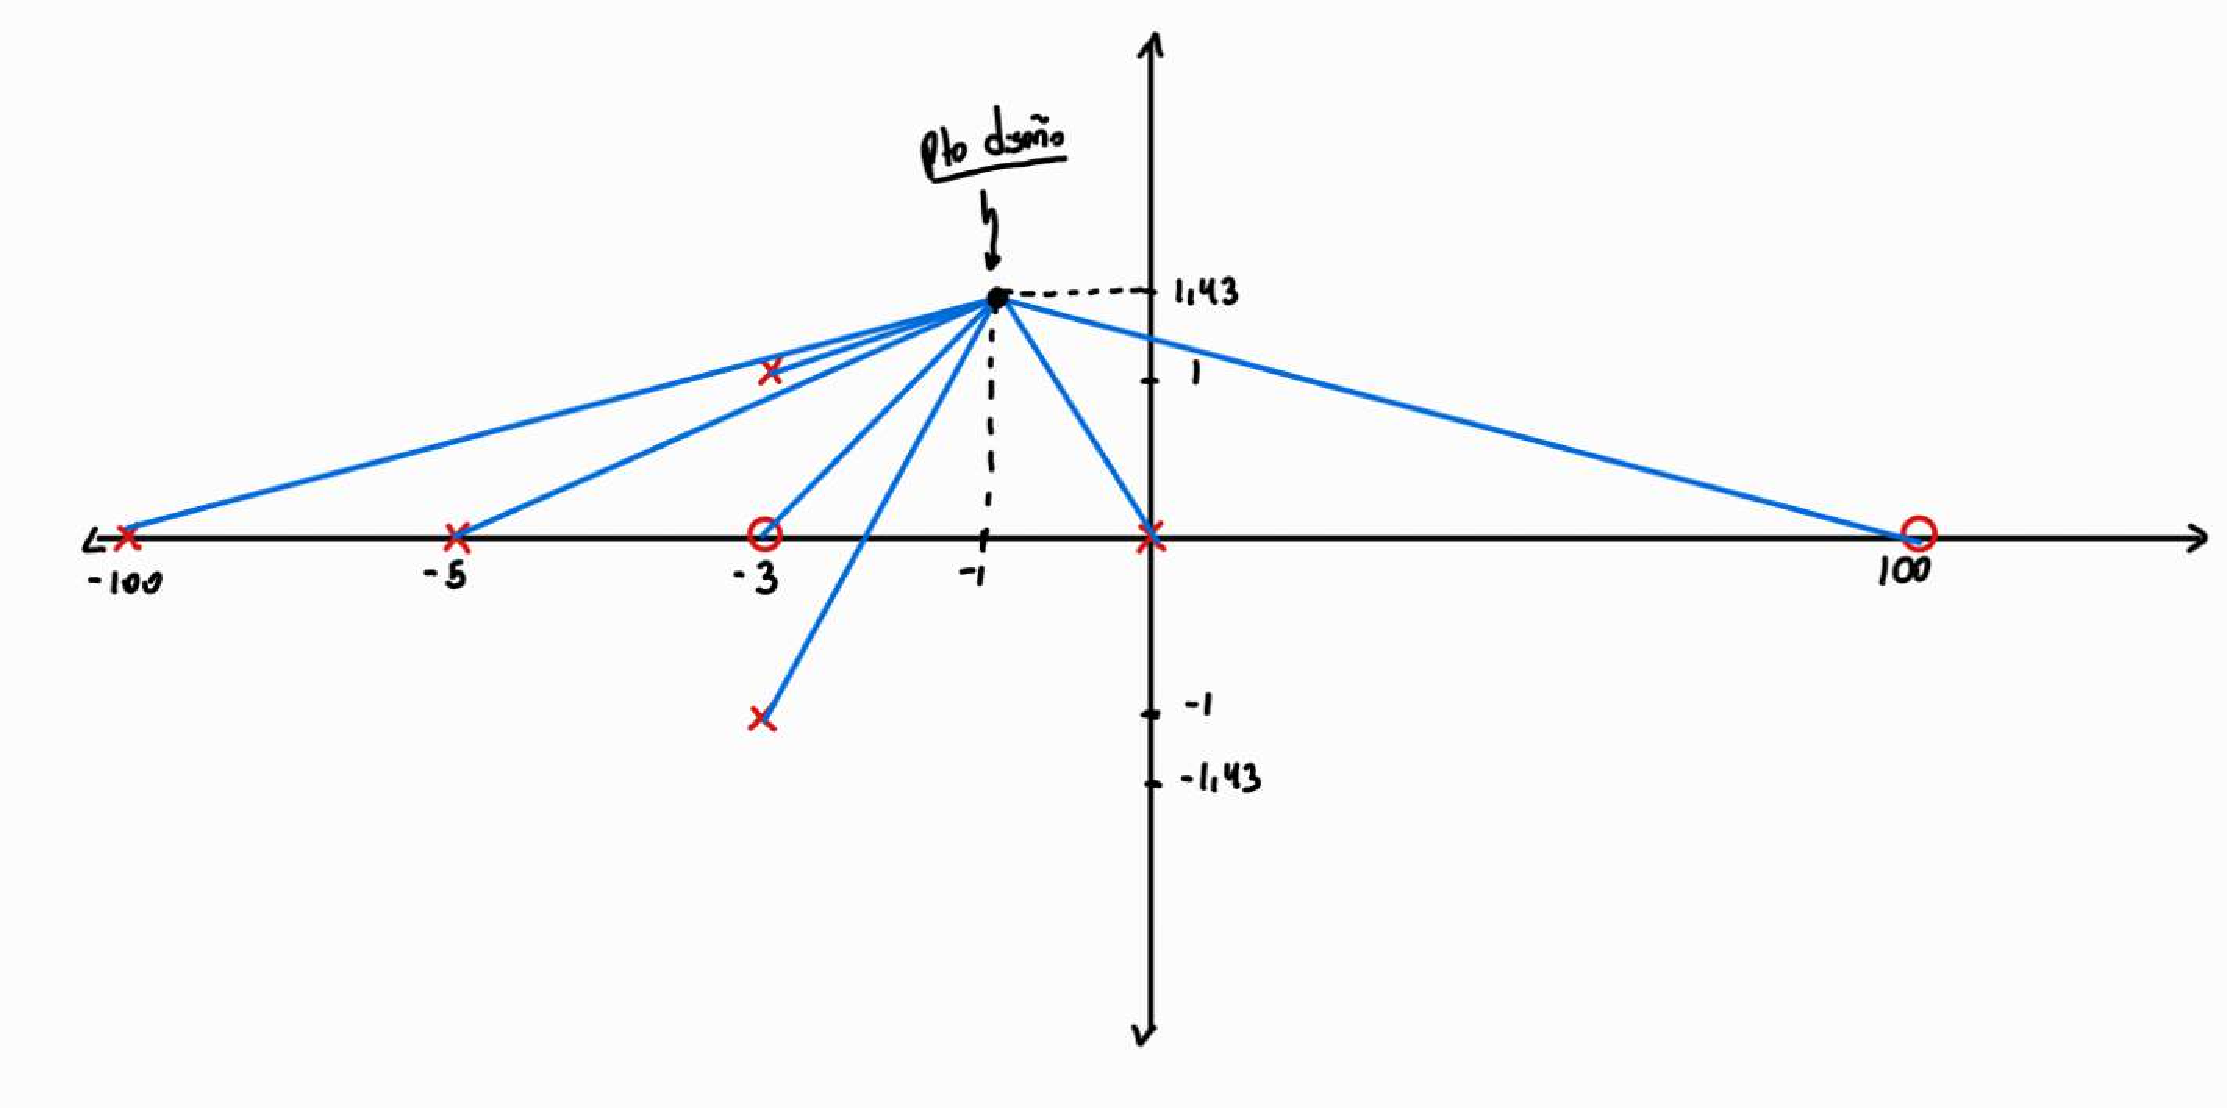
\includegraphics[width=0.7\textwidth]{Auxiliar_6_16}
    \captionof{figure}{LGR del lazo anterior considerando retardo.}
\end{center}
Notamos que se tiene el angulo obtenido antes de considerar el retardo, es decir:
\begin{align}
    \theta_{anterior} &= 185.95^{\circ}\\
    \theta_{100} &= atan\left(\frac{1.43}{100-1.4}\right) = 0.83^{\circ}\\
    \theta_{-100} &= 180^{\circ} atan\left(\frac{1.43}{100+1.4}\right) = 179.19^{\circ}
\end{align}
De esta manera tenemos que:
\begin{align}
    \sum \theta_{0} - \sum \theta_{z} = 0^{\circ}\\
    \theta_{anterior} + \theta_{100} - \theta_{-100} - \theta_{a} = 0^{\circ}\\
\end{align}
Con lo que se tiene que $\theta_{a}= 7.59$, por tanto:
\begin{align}
    tan(\theta_{a}) = \frac{1.43}{a-1.43}
\end{align}
Con lo que $a = 12.133$ ,de esta manera se obtiene el valor de a para la correcion del retardo.Finalmente se tendra que para la ganancia:
\begin{align}
    K_{c} &= \abs{\frac{1}{G_{p}(s)G_{c}(s)H(s)}}_{s=s^{*}}\\
          &= \abs{\frac{1}{\frac{16(s+3)}{(s+5)(s^{2}+6s+10)}\cdot \frac{100-s}{100+s}\cdot \frac{s+12.133}{s}}}_{s=-1.4+j1.43}\\
          &= \abs{\frac{1}{\frac{16(s+3)}{(s+5)(s^{2}+6s+10)}\cdot \frac{100-s}{100+s}\cdot \frac{s+12.133}{s}}}_{s=s^{*}}\\
          &= 0.0767
\end{align}
Finalmente se tendra que el controlador sera de la forma:
\begin{align}
    G_{c}(s) = 0.0767\frac{s+12.133}{s}
\end{align}
%----------------------------------------------
\subsection*{Resolucion 2.3}

\end{solution}
%----------------------------------------------
\question Sea el siguiente esquema(\textbf{P2 Control otoño 2024})

\begin{center}
    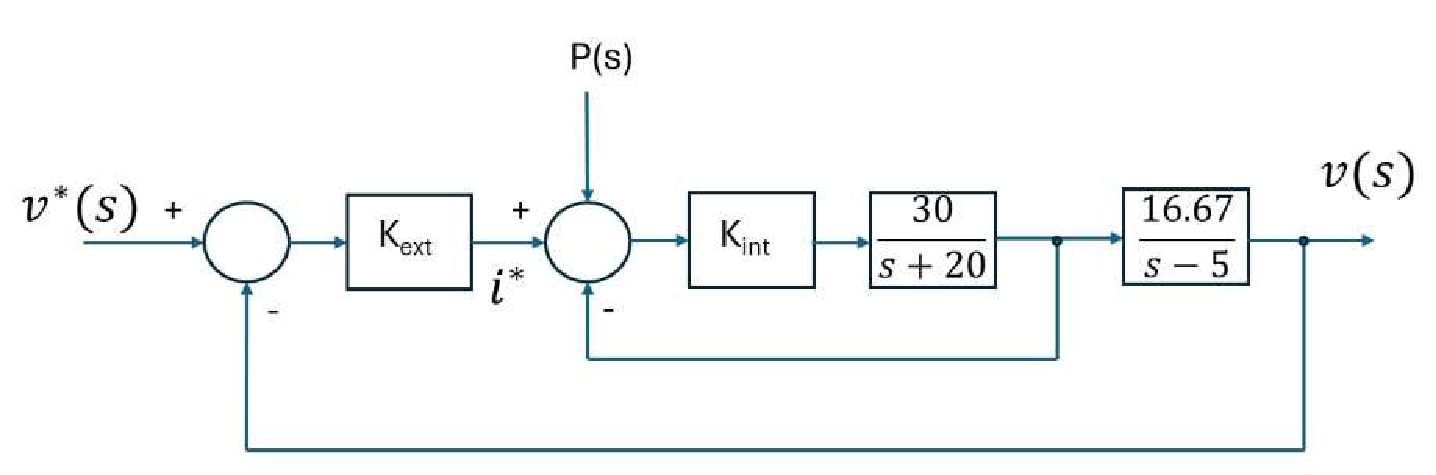
\includegraphics[width=0.8\textwidth]{Auxiliar_6_7}
    \captionof{figure}{Esquema }
\end{center}
En la figura anterior, los controladores \(K_{\text{ext}}\) y \(K_{\text{int}}\) son iguales a 1. Asuma inicialmente que \(P(s) = 0\). Los lazos son diseñados para que el lazo interno tenga una frecuencia natural de \(\omega_n = 50 \, \text{rads/seg}\) y el lazo externo quede con \(\omega_n = 5 \, \text{rads/seg}\). Es decir, se encuentran inicialmente desacoplados por velocidad de respuesta. Se pide:

\begin{enumerate}
    \item Encuentre los coeficientes de amortiguamiento de cada lazo, es decir del lazo interno y del lazo externo, para esta condición de diseño. Justifique su respuesta utilizando gráficos del lugar de la raíz y ecuaciones.
    \item ¿Los valores de los coeficientes de amortiguamiento encontrados pueden cambiar si P(s) = 3/s?. Justifique su respuesta
    \item Debido a envejecimiento, la ganancia del lazo interno comienza a cambiar de la forma $K_{int} = (1 - 0.1\cdot t)$, donde t es el tiempo en segundos Encuentre el valor de t donde se produce inestabilidad asintótica del sistema de control. Justifique su respuesta utilizando gráficos del lugar de la raíz y ecuaciones
    \item Se repara el problema ocasionado por el envejecimiento de componentes y se opera nuevamente con \(K_{\text{ext}} = K_{\text{int}} = 1\). Un ingeniero con mucha iniciativa decide que el sistema de control de la figura debe tener cero error en estado estacionario a una señal de entrada de la forma \( v^*(t) = 3t + 7\sin(2\pi 50t) \). Se pide:
    \begin{enumerate}
        \item ¿Qué componentes mínimos debería tener un controlador que cumpla con este requerimiento?.
        \item ¿Este controlador debería estar ubicado en el lazo interno, lazo externo o una com-
        binación de ambos
    \end{enumerate}

\end{enumerate}
%-----------------------------------------------
\begin{solution}
\subsection*{Resolucion 3.1}
Se busca obtener los coeficientes de amortiguamiento de cada lazo, es importante notar ademas que se encuentran desacoplados ademas que $K_{int}=K_{ext}=1$. Analizando el lazo interno tenemos solo un polo por lo que el LGR vendra dado por:
\begin{center}
    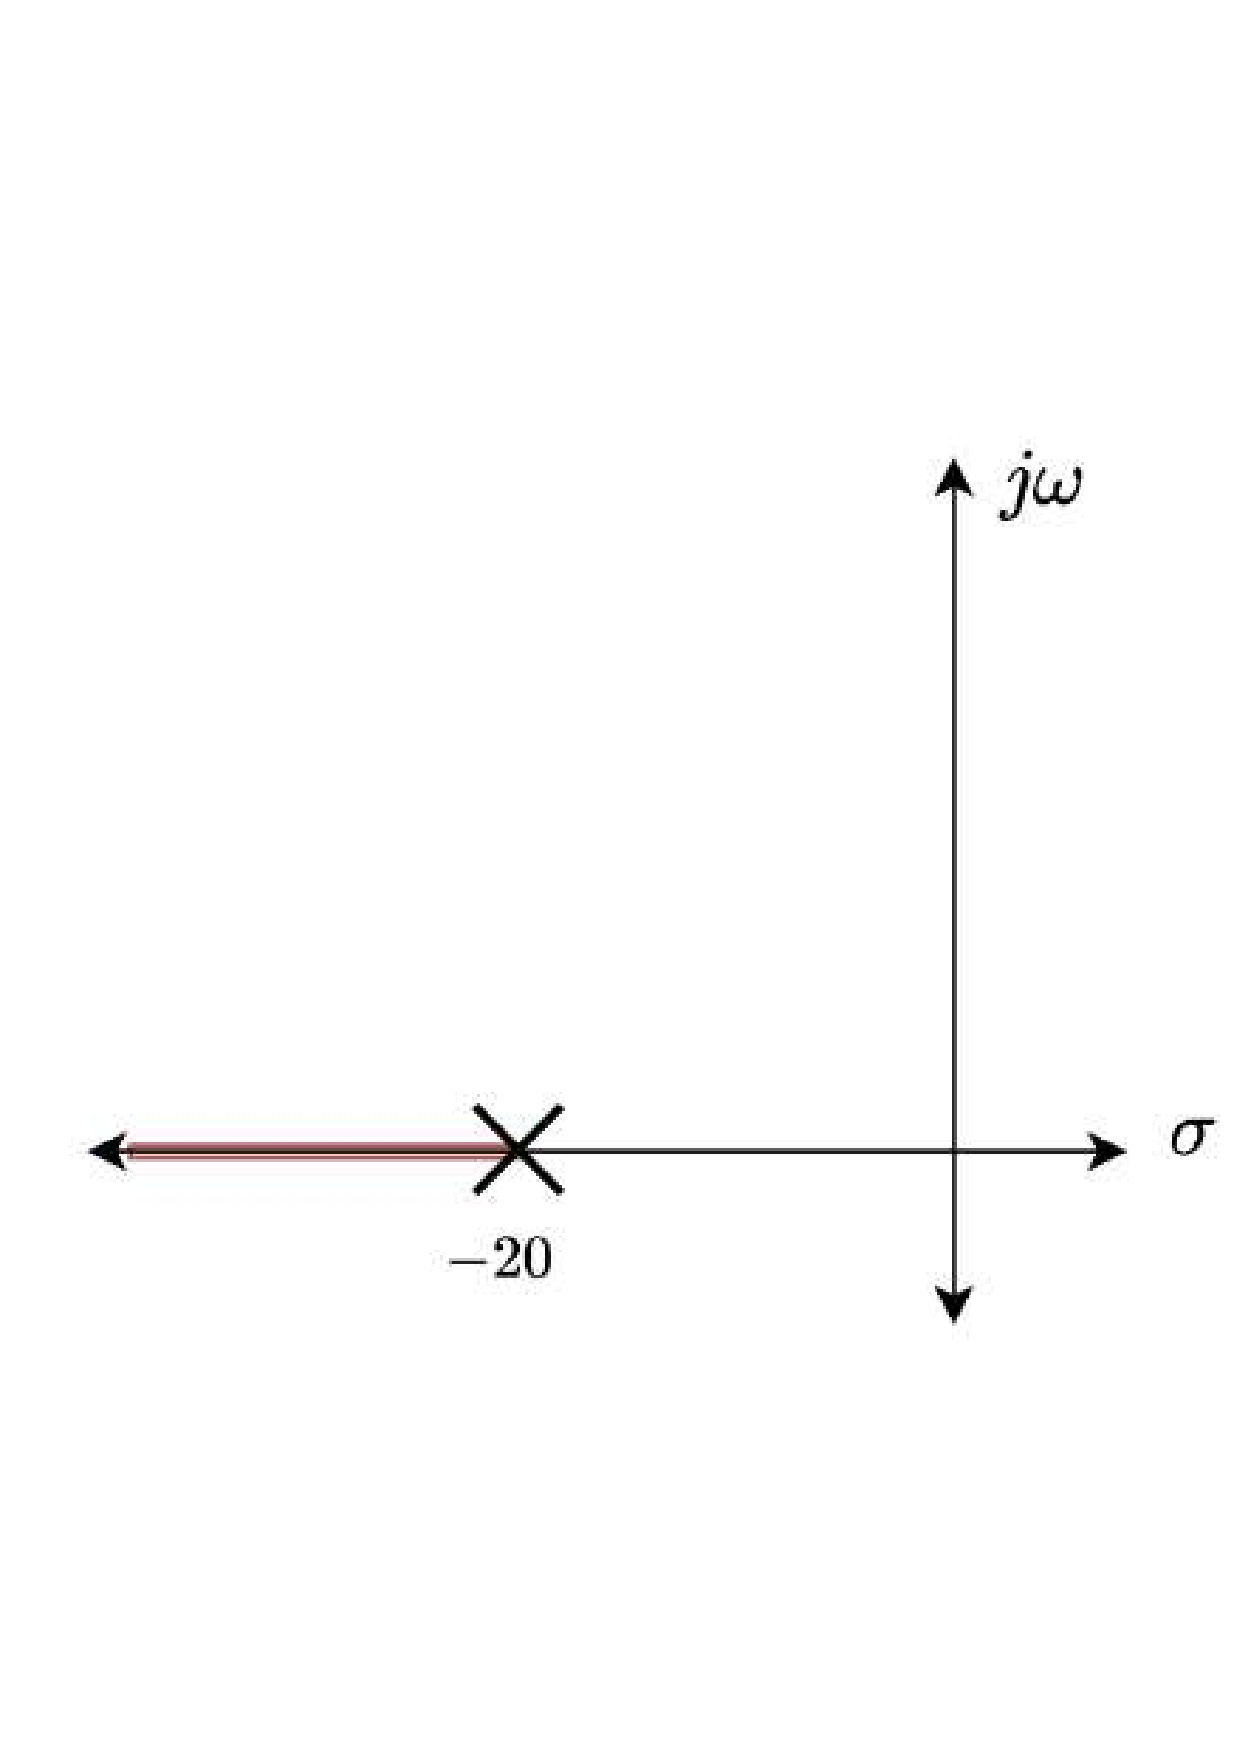
\includegraphics[width=0.3\textwidth]{Auxiliar_6_12}
    \captionof{figure}{LGR para el lazo interno}
\end{center}
Notamos que al haber solo un polo, este se encontrara unicamente en la parte real, por lo que necesariamente debera cumplir que $\zeta_{int} = 1$ ademas se puede obtener el punto de diseño para el cual esta pensado, considerando que $w_{n}=50$ rad/s, por lo que se tiene que:
\begin{align}
    s_{1,2}^{*} &= -\zeta \omega_{n} \pm j\omega_{n}\sqrt{1-\zeta^{2}}\\
    & = -50 \pm j50\sqrt{1-1}\\
    & = -50
\end{align}
Con lo que se caracteriza el lazo interno, por otro lado se tiene el lazo externo, el cual tiene nuavemente un solo polo, si bien el procedimiento a seguir es el mismo, se debe tener en consideracion que a pesar que esten desacoplados, el lazo interno podria introducir una ganancia extra que se obtiene en base al teorema del valor final. Por lo que el sistema vendria dado por:
\begin{center}
    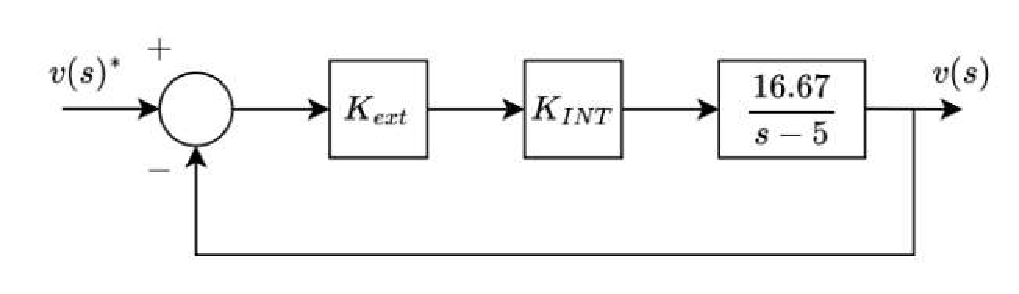
\includegraphics[width=0.65\textwidth]{Auxiliar_6_8}
    \captionof{figure}{Esquema del lazo externo el cual considera una ganancia interna asocada al teorema del valor final.}
\end{center}
Luego el LGR vendra dado por lo siguiente:
\begin{center}
    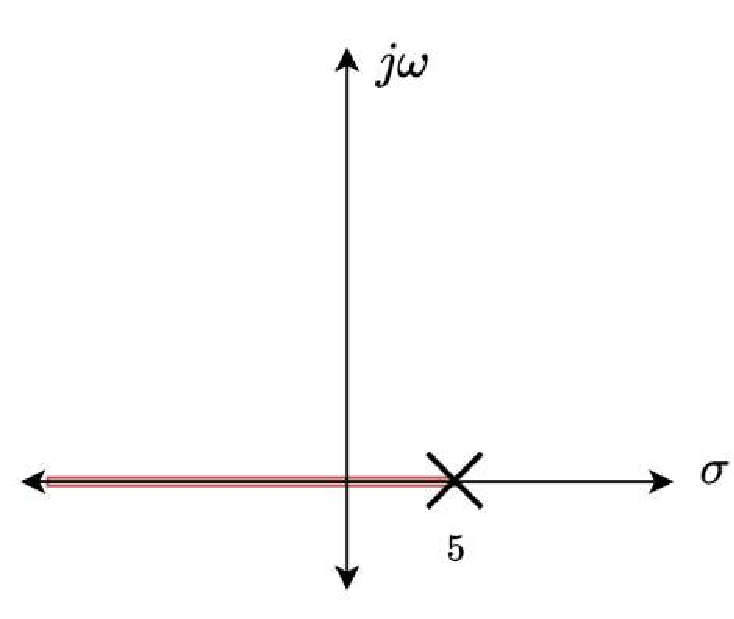
\includegraphics[width=0.3\textwidth]{Auxiliar_6_9}
    \captionof{figure}{LGR para el lazo externo}
\end{center}
Luego se tendra que el lazo externo debera tambien debera tener un coeficiente de amortiguamiento de 1 y por tanto el punto de diseño de este sera:
\begin{align}
    s_{1,2}^{*} &= -\zeta \omega_{n} \pm j\omega_{n}\sqrt{1-\zeta^{2}}\\
    & = -5 \pm j5\sqrt{1-1}\\
    & = -5
\end{align}
Con lo que se obtienee l coeficiente de amortiguamiento para ambos lazos.
%----------------------------------------------
\subsection*{Resolucion 3.2}
Se busca determinar si los valores de los coeficientes de amortiguamiento encontrados pueden cambiar si $P(s) = 3/s$, para esto recordamos los siguiente:
\begin{center}
    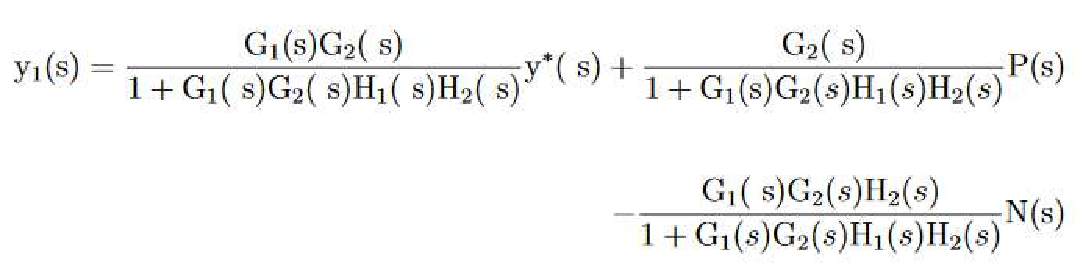
\includegraphics[width=0.65\textwidth]{Auxiliar_6_11}
    \captionof{figure}{Ecuaciones asociada a el sistema considerando tanto ruido N como perturbaciones P}
\end{center}
Notamos que la perturbacion o la entrada adicional,  no modifica los componentes principales del lazo interno, ya sea la planta o el controlador. Dado que no incide en la planta directamente, los LGR se mantienen tal y como se describieron en la pregunta anterior, por lo que la perturbación no cambia los coeficientes de amortiguamiento de ambos lazo. Pero si afectara otros aspectos del sistema.
%----------------------------------------------
\subsection*{Resolucion 3.3}
Debido al envejecimiento de la planta ahora tenemos que considerar que la planta tiene una ganancia con una dependencia temporal dada por $K_{int} = (1-0.1t)$ , para esto se utilizara el criterio de Routh-Hurwitz, por lo que primero debemos tener en cuenta que la funcion de transferencia de lazo cerrado para el lazo interno vendra dada por:
\begin{align}
    G_{int}(s) = \frac{G(s)}{1+G(s)H(s)} 
\end{align}
Que para nuestro caso particular
\begin{align}
    G_{int}(s) = \frac{30K_{int}}{s+20+30K_{int}}
\end{align}
Por lo que la ecuacion caracteristica a lazo cerrado del sistema, es decir considerando el efecto del lazo interno vendra dada por:
\begin{align}
    1+ \frac{30K_{int}}{s+20+30K_{int}} \cdot \frac{16.76}{s-5} &= 0\\
    (s+20+30K_{int})(s-5) + 30\cdot 16.76 K_{int} &= 0\\
    s^{2} + s(15+30K_{int}) + (350.1K_{int} - 100 ) &= 0\\
    s^{2} + \alpha s + \beta &= 0
\end{align}
Luego aplicado el criterio de Routh-Hurwitz se tiene que su tabla asociada:
\[
\begin{array}{|c|c|c|}
\hline
s^2 & 1 & \beta \\
\hline
s^1 & \alpha & 0 \\
\hline
s^0 & \beta & \\
\hline
\end{array}
\]
De esta manera tendremos que para que el sistema sea estable se debe cumplir que $\alpha > 0$ y $\beta > 0$, por lo que se tiene que:
\begin{align}
    \alpha &= 15 + 30K_{int} > 0\\
    30K_{int} &> -15\\
    K_{int} &> -0.5\\
    1-0.1t &> -0.5\\
    t &< \frac{1.5}{0.1}\\
\end{align}
Por lo que tenemos que el $t_{critico}$ sera igual a 15[s].Mientras que para $\beta$ se debera cumplir que:
\begin{align}
    \beta &= 350.1K_{int} - 100 > 0\\
    350.1K_{int} &> 100\\
    K_{int} &> \frac{100}{350.1}\\
    1-0.1t &> \frac{100}{350.1}\\
    t& < \left(1- \frac{100}{350.1}\right)\cdot 10\\
\end{align}
Con lo que para $\beta$ se tendra que el tiempo critico corresponde a 7.1[s]. Luego se debe tomar en cuenta el minimo valor que permita que ambos casos se cumplen simulateneamente, por lo tanto tendremos que el tiempo critico sera igual a 7.1s.\\\\
Otra manera valida de resolver el problema es mediante el teorema de valor final para una entrada escalon
%----------------------------------------------
\subsection*{Resolucion 3.4}
\subsubsection*{Resolucion 3.4.1}
Se busca obtener los componentes minimos que permitan que el sistema tenga cero error en estado estacionario, para esto se debe tener en cuenta que la señal de entrada vendra dada por:
\begin{align}
    v^{*}(t) = 3t + 7\sin(2\pi 50t)
\end{align}
Por lo que al pasar al dominio de laplace tenemos que:
\begin{align}
    V^{*}(s) &= \frac{3}{s^{2}} + \frac{7\cdot 2\pi 50}{s^{2} + (2\pi 50)^{2}}\\
             &= \frac{3(s^{2} +(2\pi50)^{2} + s^{2} 7 \cdot 2 \pi 50) }{s^{2}( s^{2} + (2\pi 50)^{2})}
\end{align}
Por lo que el controlador debera almenos poseer en su denominador el termino $s^{2}( s^{2} + (2\pi 50)^{2})$, para que tener cero error a estado estacionario.\\\\
Dare otro ejemplo para que se logre entender de mejor manera, supongamos que tenemos una planta $G_{p}$ luego tenemos que el teorema del valor final viene dado por:
\begin{align}
    lim_{t\to \infty} e(t) = lim_{s\to 0} se(s) &= \frac{u(s)}{1+G_{c}(s)G_{p}(s)}\\
\end{align}
Por lo que si suponemos una entrada escalon la cual viene dada por $U(s)= \frac{1}{s}$ luego se tendra que:
\begin{align}
    lim_{s\to 0} se(s) &= \frac{s \cdot \frac{1}{s}}{(1+ \frac{K}{s}G(s))}= 0
\end{align}
Luego vemos que el controlador debera tener almenos en el denominador el mismo termino que la entrada,dado que de esta forma el limite anterior sera 0 y podremos asegurar 0 error a estado estacionario.
%----------------------------------------------
\subsubsection*{Resolucion 3.4.2}
Este controlador debería ubicarse en el lazo externo del sistema de control, dado que el desacople de los mismos hace que cuando el sistema se someta a esta entrada, solo
las dinámicas del lazo externo serán las relevantes. Esto es porque el lazo interno puede representarse como una ganancia en régimen permanente, lo cual no afecta en estado estacionario a la sintonización del controlador.
%----------------------------------------------
\end{solution}
\end{questions}
\newpage
%%%%%%%%%%%%%%%%%%%%%%%%%%%

\end{document}